\documentclass[3p,times,single-column]{elsarticle}

% Encoding and fonts
\usepackage[T1]{fontenc}
\usepackage[utf8]{inputenc}
\usepackage{lmodern}
\renewcommand{\ttdefault}{lmtt}

% Layout and tables
\usepackage{booktabs}
\usepackage{array}
\usepackage{pdflscape}

% Math and graphics
\usepackage{amsmath}
\usepackage{amssymb}
\usepackage{graphicx}

% Links
\usepackage{hyperref}

\journal{Environmental Modelling \& Software}

\begin{document}

\begin{frontmatter}

\title{Variance Retention: A Forecast-Verification Diagnostic for\\Skilful-but-Smoothed Point Forecasts of Daily PM$_{10}$}

\author[1]{Federico Garc\'ia Crespi\corref{cor1}}
\ead{fedeg@umh.es}

\author[2]{Julio Alberto Ramos Mart\'inez}
\ead{j.ramos@umh.es}

\cortext[cor1]{Corresponding author}
\affiliation[1]{organization={Department of Computer Engineering, Universidad Miguel Hern\'andez},city={Elche},country={Spain}}
\affiliation[2]{organization={Department of Statistics, Mathematics and Computer Science, Universidad Miguel Hern\'andez},city={Elche},country={Spain}}

\begin{abstract}
Environmental forecasts can improve on a persistence reference while
preserving less of the observed dynamic variation. We examined whether
making that distinction explicit changes the set of station--model--horizon
cells passing a post-evaluation screening audit in a rolling-origin
benchmark of daily PM$_{10}$ forecasts from 17 Spanish monitoring stations,
five model families, and seven horizons. Across 595 structured cells, Rule A
required positive persistence-relative RMSE skill and a significant
comparison with persistence; Rule B added study-specific heuristic
thresholds for variance retention and P75 exceedance recall. Rule A retained
277 cells, whereas Rule B retained 8, so 269 cells changed status (97.1\% of
Rule-A cells).
A threshold sensitivity analysis found that 91.3--98.2\% of Rule-A cells
changed across the tested neighbourhood. The results show that error and
dynamic fidelity can produce different cell-screening outcomes under these
stated rules; the magnitude is conditional on this pollutant, benchmark, and
validation design. Here, eligibility denotes only passage of the stated
post-evaluation cell screen, not model ranking or operational acceptance.
\end{abstract}


\begin{keyword}
forecast verification \sep deterministic point forecasts \sep PM$_{10}$ forecasting \sep rolling-origin evaluation \sep persistence baseline \sep variance retention \sep exceedance diagnostics
\end{keyword}

\end{frontmatter}

\section{Introduction}
\label{sec:introduction}

Environmental forecasting supports decisions that depend on both expected error and the timing or amplitude of changing conditions. A candidate forecast is therefore commonly compared with a meaningful reference forecast, rather than judged only by an isolated error value. Persistence-relative skill provides such a comparison for daily time series, while formal predictive-accuracy tests can assess whether an observed loss difference is statistically distinguishable from the reference \cite{hyndman2006,diebold1995}.

These error-based summaries are necessary but not exhaustive. A point forecast may reduce average squared error by attenuating fluctuations, particularly when the future is uncertain. Lower error can therefore coexist with a forecast trajectory whose variance or episode amplitude is smaller than that of the observations. Forecast verification distinguishes accuracy, association, calibration, and related properties because no single summary answers all of these questions \cite{gneiting2011,jolliffe2012}.

The distinction matters when evaluation results are converted into eligibility decisions. A cell that improves on persistence under RMSE may remain unsuitable for a decision that requires sensitivity to elevated pollution or preservation of dynamic spread. Variance and event diagnostics are established complements to error measures; they are not introduced here as new metrics. The unresolved practical issue is whether adding explicit fidelity requirements to an error-based eligibility rule materially changes the set of cells that pass.

The EMS audit motivating this study supports a deliberately bounded gap. Existing environmental forecasting studies commonly evaluate predictive error and, less consistently, dynamic-fidelity dimensions, while evidence remains limited on whether explicitly combining these dimensions in an eligibility rule materially changes decisions across sites, model families, and forecast horizons. This statement describes the audited corpus; it does not claim that no such study exists elsewhere.

We ask: \emph{Does incorporating dynamic-fidelity criteria alongside conventional error-based statistical evaluation materially alter model eligibility in multi-step daily PM$_{10}$ forecasting?} We answer with a post-evaluation audit of a fixed multi-station benchmark. The contributions are:
\begin{enumerate}
    \item an empirical audit of error--fidelity discordance;
    \item a characterisation of its variation across model families and horizons; and
    \item a quantification of how explicit fidelity requirements alter eligibility.
\end{enumerate}

\section{Evaluation Context and EMS Gap}
\label{sec:background}

Reviews of air-quality forecasting report substantial use of RMSE, MAE, correlation, and related point-error summaries when comparing statistical and machine-learning models \cite{mendez2023,tang2024,chadalavada2025}. These summaries are informative, but reporting of forecast variability and event sensitivity is less consistent in the audited literature.

Rolling-origin evaluation is established for time-series forecasting because it preserves temporal ordering and limits information leakage \cite{tashman2000,bergmeir2018}. Yet a leakage-free evaluation can still be decisionally one-dimensional if eligibility is determined only by error. The gap addressed here is therefore narrow: evidence is limited on whether explicitly combining error and dynamic-fidelity dimensions materially changes eligibility across sites, model families, and horizons. This is an audit of decision consequences, not a claim that the underlying metrics or the broader literature are new.

\section{Decision Audit Framework}
\label{sec:framework}

We compare two eligibility rules applied after forecast evaluation. The rules do not retrain models or create a new ranking objective; they audit how a stated requirement changes the set of eligible cells.

\subsection{Error-based eligibility: Rule A}
For each station--model--horizon cell,
\begin{equation}
\textbf{Rule A:}\qquad \mathrm{Skill}>0 \quad\mathrm{and}\quad \mathrm{DM}_{BH}\ \text{significant}.
\end{equation}
Skill is persistence-relative RMSE skill. The significance flag is based on the two-sided Harvey--Leybourne--Newbold modified Diebold--Mariano comparison with Benjamini--Hochberg adjustment, as implemented in \texttt{scripts/05\_dm\_significance.py} \cite{diebold1995,harvey1997}.

\subsection{Fidelity-aware eligibility: Rule B}
\begin{equation}
\textbf{Rule B:}\qquad \text{Rule A}\quad\mathrm{and}\quad \alpha\geq0.50\quad\mathrm{and}\quad \mathrm{Recall}_{P75}\geq0.20.
\end{equation}
The two thresholds are operational criteria chosen for this audit. They are not estimated optima, universal standards, or claims about acceptable performance in other applications. A decision change is a cell that satisfies Rule A but not Rule B.

We also define a descriptive discordant case as a Rule-A cell with $\mathrm{Recall}_{P75}\geq0.20$ and $\alpha<0.50$. This isolates cells that pass the error and episode-sensitivity checks while failing the variance-retention check.

\section{Methods: empirical benchmark}
\label{sec:casestudy}

The study evaluates a fixed benchmark of daily PM$_{10}$ point forecasts.
The unit of analysis is a station--model--horizon cell, and the analysis
is deliberately post-evaluation: it audits how eligibility changes when
dynamic-fidelity requirements are added to an error-based screen. This
design keeps the empirical question separate from any attempt to optimise
a forecasting model.

\subsection{Data, forecast task and validation}

The frozen evidence comprises daily PM$_{10}$ series from 17 Spanish
monitoring stations identified in MITECO/EMEP metadata. The stations span
urban, traffic, industrial, suburban, and rural settings. The recovered
station package does not establish one defensible common calendar endpoint
for the complete set, so we report the verified station coverage and daily
resolution rather than infer a period label. The complete grid contains
17 stations, five empirical model families, and seven forecast horizons,
giving 595 structured rows. These rows share stations and underlying time
series; they are evaluation cells, not independent replicates.

The task is direct multi-step daily point forecasting at horizons
$h=1,\ldots,7$. Evaluation follows five expanding rolling-origin folds in
chronological order. For each origin, information that became available
after the origin was excluded from fitting, feature construction,
preprocessing, threshold estimation, and verification inputs. Missing
verification targets were excluded rather than fabricated. The frozen
aggregate does not recover exact per-fold row counts or one complete
train/test calendar, and those details are therefore not asserted.

\subsection{Forecasting models and reference forecast}

The benchmark contains five empirical model families: direct Histogram
Gradient Boosting (HGB), direct Ridge regression, fixed-order SARIMA,
seasonal naive, and STL+Ridge. HGB and Ridge produce direct forecasts for
each horizon. SARIMA is treated as a recursive statistical family,
seasonal naive as a seasonal carry-forward reference, and STL+Ridge as a
decomposition/regression hybrid. The model evaluation specification table
records the inputs and the
configuration details that can be verified from the frozen provenance.

Exact HGB, Ridge, and STL settings are not recoverable from the frozen
release. Historical SARIMA records also conflict; accordingly, we do not
invent an exact order and describe only the fixed-order family supported by
the evaluation package. This limitation affects reconstruction detail,
not the frozen aggregate diagnostics reported here.

Persistence supplies the operational comparator. It is evaluated on the
same matched forecast cases as each candidate model, so positive skill means
that the candidate reduces RMSE relative to persistence on the relevant
cell. The comparator is a reference for the eligibility audit, not a claim
that persistence is the only meaningful baseline.

\begin{table}[ht]
\centering
\scriptsize
\setlength{\tabcolsep}{2pt}
\textbf{Supplementary Table S2. Model evaluation specification.} Reconstructed from the analysis provenance. ``Not recoverable'' denotes a detail not established by the provenance; it is not inferred from model names.\par\smallskip
\begin{tabular}{@{}p{2.15cm}p{2.25cm}p{2.25cm}p{2.05cm}p{2.25cm}p{2.45cm}@{}}
\toprule
Model & Inputs & Forecast strategy & Fold fitting & Verified configuration & Known limitation \\
\midrule
HGB direct & Direct lag-based predictors; complete feature list not recoverable & One direct forecast per horizon & Fit within rolling-origin training data & Family label and 7-horizon evaluation verified & Exact hyperparameters not recoverable from frozen provenance \\
Ridge direct & Direct lag-based predictors; complete feature list not recoverable & One direct forecast per horizon & Fit within rolling-origin training data & Family label and 7-horizon evaluation verified & Exact regularisation and feature list not recoverable \\
SARIMA & Daily PM$_{10}$ series & Recursive statistical forecast & Fit within rolling-origin training data & Fixed-order SARIMA family verified & Historical configuration records conflict; exact order omitted \\
Seasonal naive & Historical seasonal observations & Seasonal carry-forward baseline & No parameter fitting beyond training history & Family label and 7-horizon evaluation verified & Seasonal period details not recoverable from canonical table \\
STL+Ridge & Decomposition and regression inputs & Hybrid decomposition/regression forecast & Fit within rolling-origin training data & Family label and 7-horizon evaluation verified & Exact STL and Ridge settings not recoverable \\
\bottomrule
\end{tabular}
\end{table}


\section{Metrics and Diagnostic Categories}

\subsection{Persistence-relative skill}
Let \(y_h\) denote the verifying observation at horizon \(h\), and \(\hat{y}_h\) the corresponding point forecast produced by a model. Let \(\hat{y}^{(p)}_h\) denote the persistence baseline forecast for the same horizon. For a chosen loss function \(L(\cdot,\cdot)\), the baseline-relative (persistence-relative) skill score at horizon \(h\) is
\begin{equation}
\mathrm{Skill}(h) = 1 - \frac{\mathbb{E}[L(y_h,\hat{y}_h)]}{\mathbb{E}[L(y_h,\hat{y}^{(p)}_h)]}.
\end{equation}
In this work, the empirical results use an RMSE-based loss, so \(\mathrm{Skill}(h)>0\) indicates a lower RMSE than persistence for the same horizon and evaluation sample \cite{hyndman2006}.

Persistence-relative skill is useful because it anchors interpretation to an operationally meaningful comparator rather than to a model-to-model ranking alone. It also supports horizon-wise reading: in multi-step settings, skill can vary substantially across lead times.

At the same time, skill is a summary of pointwise error behaviour under a chosen loss. It does not, by itself, describe the trajectory shape of the point forecasts, and it does not indicate whether an apparent improvement is associated with reduced dynamic variability.

\subsection{Variance retention}
We define the variance-retention ratio at horizon \(h\) as
\begin{equation}
\alpha(h) = \frac{\sigma^2_{\hat{y}_h}}{\sigma^2_{y_h}}
          = \frac{\operatorname{Var}(\hat{y}_h)}{\operatorname{Var}(y_h)},
\end{equation}
the ratio of the predicted to the observed \emph{variance} at horizon \(h\).
Both variances are population variances (\(\mathrm{ddof}=0\)) computed over the
matched finite forecast--observation pairs within each station--model--horizon
cell, so \(\alpha(h)\) is the fraction of observed variance retained by the
forecast (a value of \(0.5\) corresponds to half the observed variance
retained). This is a variance ratio, not a standard-deviation ratio; the two
differ by a square and are not interchangeable.

The ratio \(\alpha(h)\) compares forecast trajectory variability with observed variability at the same horizon. Values \(\alpha(h)\ll 1\) indicate variance shrinkage consistent with smoothed point-forecast trajectories, while values \(\alpha(h)\gg 1\) indicate forecast variance inflation.

Variance retention should not be interpreted as a complete measure of trajectory quality. A forecast may retain the observed variance and still be biased, phase-shifted, or poor at reproducing individual episodes. The diagnostic is therefore intended to detect one specific failure mode—variance shrinkage—rather than to certify full dynamic adequacy.

Variance retention is not a calibration measure and is not intended to assess probabilistic uncertainty. It is a bounded post-evaluation diagnostic for reading point forecasts when operational interpretation depends on day-to-day fluctuations as well as on average accuracy \cite{jolliffe2012}.

\subsection{Auxiliary \texorpdfstring{\(\mathrm{Skill}_{VP}\)}{Skill\_VP}}
To summarise the joint behaviour of baseline-relative accuracy and variance retention, we also report an auxiliary variance-penalised skill diagnostic
\begin{equation}
\mathrm{Skill}_{VP}(h) = \mathrm{Skill}(h)\cdot\alpha(h).
\end{equation}

The auxiliary diagnostic is intended to highlight cases where positive persistence-relative skill co-occurs with strong variance shrinkage. The product form is not claimed to be uniquely optimal; it is used here only as a transparent descriptive penalty that keeps the sign of \(\mathrm{Skill}(h)\) while reducing positive skill when forecast variance is strongly collapsed. It should not be interpreted as a replacement for standard accuracy metrics, uncertainty quantification, or statistical significance testing \cite{diebold1995}.

Accordingly, \(\mathrm{Skill}_{VP}(h)\) is used only as a bounded diagnostic layer for post-evaluation interpretation. Its role is to provide a compact joint summary alongside \(\mathrm{Skill}(h)\) and \(\alpha(h)\), rather than to define a universal performance criterion.

\subsection{Diagnostic flags}
In addition to \(\alpha(h)\) and \(\mathrm{Skill}_{VP}(h)\), the post-evaluation reports diagnose flags for horizon-wise interpretation. The \texttt{collapse\_flag} is used when \(\alpha(h) < 0.5\). The \texttt{inflation\_flag} is used when \(\alpha(h) > 1.5\). The \texttt{near\_ideal\_flag} is used when \(\mathrm{Skill}(h)>0\) and \(0.8 \leq \alpha(h) \leq 1.2\). The \texttt{low\_sample\_flag} indicates fewer than 30 verification samples for a model/horizon cell.

These thresholds are diagnostic conventions for this post-evaluation, not universal decision rules. A collapse flag does not invalidate a model, and an inflation flag does not imply a better dynamic representation; the flags are intended to make horizon-wise interpretation auditable and reproducible.


\section{Evidence governance and reproducibility}
\label{sec:workflow}

The empirical analysis is governed by a frozen 595-row diagnostic table
whose SHA-256 is recorded in the provenance manifest. That table contains
the complete five-model, 17-station, seven-horizon grid and is the sole
source for the numerical results, tables, and scientific figures in this
manuscript. The result-set manifest records the role and provenance of each
displayed element.

Reproducibility has two layers. The scientific layer defines the forecast
task, temporal validation, metrics, eligibility rules, and limitations. The
computational layer preserves source tables, deterministic generators,
integrity checks, and claim-level traceability. Internal audit material is
not required to compile the manuscript and is excluded from the submission
archive.

The threshold analysis is a deterministic transformation of the frozen
rows. It changes neither forecasts nor the primary thresholds. Its purpose
is to test whether the eligibility consequence persists in the prespecified
neighbourhood $\alpha\in\{0.40,0.50,0.60\}$ and
$\mathrm{Recall}_{P75}\in\{0.10,0.20,0.30\}$; it is not a threshold-optimisation
exercise.

\section{Results}

\subsection{Five-model diagnostic summary}
\label{sec:results_five_model_summary}

Across 17 stations and seven forecast horizons, direct HGB and Ridge achieve positive RMSE skill in all station-horizon cells but show near-universal variance collapse. HGB collapses in 118/119 cells (99.2\%) and Ridge in 118/119 cells (99.2\%), with only two $h=1$ point-estimate exceptions: Huesca for HGB ($\alpha = 0.544$) and Barcelona Vall d'Hebron for Ridge ($\alpha = 0.502$). SARIMA exhibits a similar but slightly less extreme pattern, collapsing in 110/119 cells (92.4\%). Seasonal naive preserves variance (0/119 collapsed cells) but has slightly negative median skill, whereas STL+Ridge avoids variance collapse but inflates variability and performs substantially worse in RMSE skill. Thus, the observed trade-off is not a simple model ranking problem: models can be significantly skillful in RMSE while dynamically over-smoothed, or dynamically variable while inaccurate.

\begin{landscape}
\begin{table}[p]
\centering
\small
\setlength{\tabcolsep}{5pt}
\caption{Model-family diagnostic summary across 17 stations and seven horizons. Collapse is defined as $\alpha < 0.5$. Near-ideal cells require positive RMSE skill and $\alpha \geq 0.8$. DM counts report BH-adjusted Diebold-Mariano tests against persistence. Exceedance metrics summarize event-detection behaviour across the evaluated thresholds.}
\label{tab:five_model_diagnostic_summary}
\begin{tabular}{llrrrrrrrrr}
\toprule
Model & Family & Med. Skill & Med. $\alpha$ & Collapse \% & Retained \% & Near-Ideal \% & Sig. Imp & Sig. Deg & Med. CSI & Med. FAR \\
\midrule
hgb\_direct & Direct ML & 0.205 & 0.151 & 99.2\% & 0.0\% & 0.0\% & 111 & 0 & 0.121 & 0.647 \\
ridge\_direct & Direct ML & 0.219 & 0.087 & 99.2\% & 0.0\% & 0.0\% & 117 & 0 & 0.104 & 0.595 \\
sarima & Statistical baseline & 0.208 & 0.095 & 92.4\% & 0.0\% & 0.0\% & 44 & 0 & 0.118 & 0.500 \\
seasonal\_naive & Variance-preserving naive & -0.026 & 1.000 & 0.0\% & 98.3\% & 16.8\% & 5 & 34 & 0.111 & 0.822 \\
stl\_ridge\_direct & Decomposition + Ridge & -1.107 & 1.399 & 0.0\% & 100.0\% & 0.0\% & 0 & 119 & 0.104 & 0.896 \\
\bottomrule
\end{tabular}
\end{table}
\end{landscape}


Under the ``near-ideal'' criterion (Skill $>0$ and $\alpha \geq 0.8$), no non-naive evaluated model attains any near-ideal cell: HGB direct, Ridge direct, SARIMA, and STL+Ridge each have 0/119 near-ideal cells. Seasonal naive contributes 20/119 near-ideal cells, but it is a naive reference and should not be interpreted as a superior predictive model.

\subsection{Horizon profiles of skill and variance retention}

To make the multi-horizon behaviour readable in the main text, we summarise horizon profiles using station-wise medians and interquartile ranges (IQR). Figure~\ref{fig:skill_profiles} reports median persistence-relative RMSE skill by horizon, and Figure~\ref{fig:alpha_profiles} reports the corresponding variance-retention ratio $\alpha$. The detailed three-model horizon table used in early diagnostic development is provided in the Supplementary Material.

\begin{figure}[t]
  \centering
  
\includegraphics[width=\linewidth]{figures/figure3_skill_profiles.pdf}
  \caption{Median persistence-relative RMSE skill by forecast horizon across 17 PM$_{10}$ stations. Shaded bands denote interquartile ranges across stations. HGB, Ridge, and SARIMA retain positive median skill, whereas seasonal naive remains close to persistence and STL+Ridge is substantially worse than persistence.}
  \label{fig:skill_profiles}
\end{figure}

\begin{figure}[t]
  \centering
  
\includegraphics[width=\linewidth]{figures/figure4_alpha_profiles.pdf}
  \caption{Median variance-retention ratio by forecast horizon across 17 PM$_{10}$ stations. The grey region indicates collapsed variance ($\alpha < 0.5$), and the green band indicates near-retained variance. HGB, Ridge, and SARIMA rapidly enter the collapsed region, while seasonal naive remains close to $\alpha = 1$ and STL+Ridge preserves or inflates variance.}
  \label{fig:alpha_profiles}
\end{figure}

\subsection{Skill--$\alpha$ diagnostic space}

Figure~\ref{fig:skill_alpha_space} provides a single-reading diagnostic summary of the skill--fidelity trade-off (cf. joint-performance summaries in \cite{taylor2001}).

\begin{figure}[t]
  \centering
  
\includegraphics[width=\linewidth]{figures/figure5_scatter_skill_alpha.pdf}
  \caption{Skill-retention diagnostic by model. Points show model-level medians across station-horizon cells, and error bars show interquartile ranges. HGB, Ridge, and SARIMA occupy the skillful-but-collapsed region, seasonal naive lies near retained variance but near-zero skill, and STL+Ridge preserves or inflates variance while losing RMSE skill.}
  \label{fig:skill_alpha_space}
\end{figure}

\subsection{SARIMA and STL+Ridge as diagnostic controls}

SARIMA and STL+Ridge were included to test whether the skill--variance trade-off is specific to direct lag-only ML. SARIMA behaves similarly to HGB and Ridge: it obtains positive median RMSE skill (0.208) but collapses in 110/119 cells (92.4\%). STL+Ridge provides the opposite control case. It avoids variance collapse in all cells and has median $\alpha = 1.399$, but its median RMSE skill is strongly negative ($-1.107$) and all 119 station-horizon cells are significantly worse than persistence under the BH-adjusted DM test. This result shows that preserving amplitude is necessary but not sufficient: the retained variability must also be phase-aligned and forecast-relevant.

\subsection{Sensitivity to the $\alpha$ threshold}

The conclusion is robust to threshold perturbations. At $\alpha < 0.4$, HGB and Ridge still collapse in 92.4\% and 89.9\% of cells, respectively; at $\alpha < 0.5$ both collapse in 99.2\%; and at $\alpha < 0.6$ both collapse in 100.0\%. SARIMA also remains highly collapsed across this range (89.9\%, 92.4\%, and 96.6\%, respectively). Seasonal naive and STL+Ridge remain non-collapsed at these thresholds. The threshold $\alpha = 0.5$ is therefore not driving the qualitative conclusion, although it should be interpreted as a diagnostic convention rather than a universal physical boundary.

\begin{figure}[t]
  \centering
  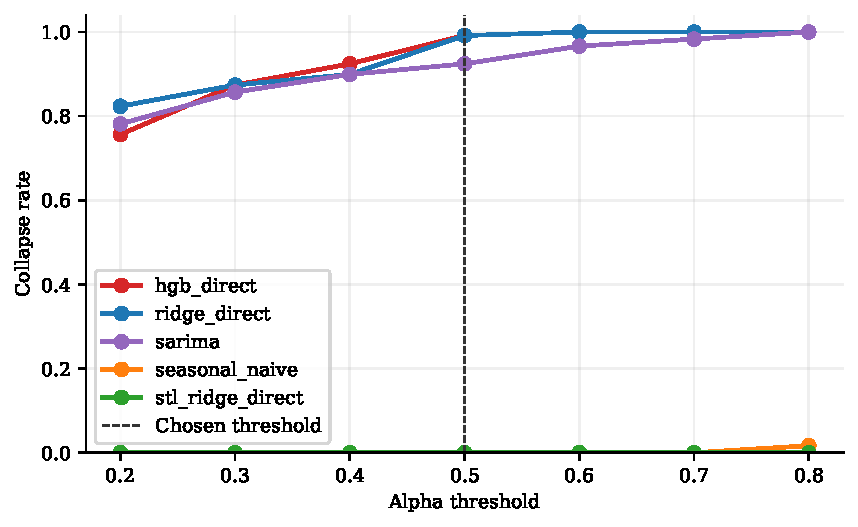
\includegraphics[width=\linewidth]{figures/figure_threshold_sensitivity.pdf}
  \caption{Sensitivity of the variance-collapse diagnostic to the $\alpha$ threshold. Collapse remains near-universal for HGB and Ridge across reasonable thresholds around $\alpha = 0.5$, and SARIMA follows the same qualitative pattern. Seasonal naive and STL+Ridge remain non-collapsed over the same range, showing that the diagnostic separates smoothed forecasts from variance-preserving or variance-inflating alternatives.}
  \label{fig:threshold_sensitivity}
\end{figure}

\subsection{Diebold--Mariano significance against persistence}

The RMSE gains of the smoothed models are not merely sampling noise. Relative to persistence, the BH-adjusted Diebold--Mariano tests (paired squared losses with the Harvey--Leybourne--Newbold correction \cite{harvey1997}) identify significant improvements in 111/119 HGB cells and 117/119 Ridge cells. SARIMA is significantly better in 44/119 cells. In contrast, STL+Ridge is significantly worse in all 119 cells. These tests make the central paradox explicit: statistically significant RMSE improvements can coexist with severe loss of predictive variance and poor event sensitivity.

\subsection{Operational consequence: exceedance behaviour}

The operational consequence of variance collapse is visible in event detection. For P75 events, mean recall is 26.9\% for HGB, 21.0\% for Ridge, and 15.6\% for SARIMA, compared with 40.0\% for persistence and 32.6\% for seasonal naive. At P90, recall falls to 7.4\%, 5.6\%, and 6.9\%, respectively. STL+Ridge achieves much higher recall (98.4\% at P75 and 87.7\% at P90), but with low precision (mean 24.2\% at P75) and high false-alarm rates. Thus, neither RMSE skill nor variance retention alone is sufficient for operational forecasting: the evaluation must jointly consider amplitude, event detection, and false alarms.

\begin{figure}[t]
  \centering
  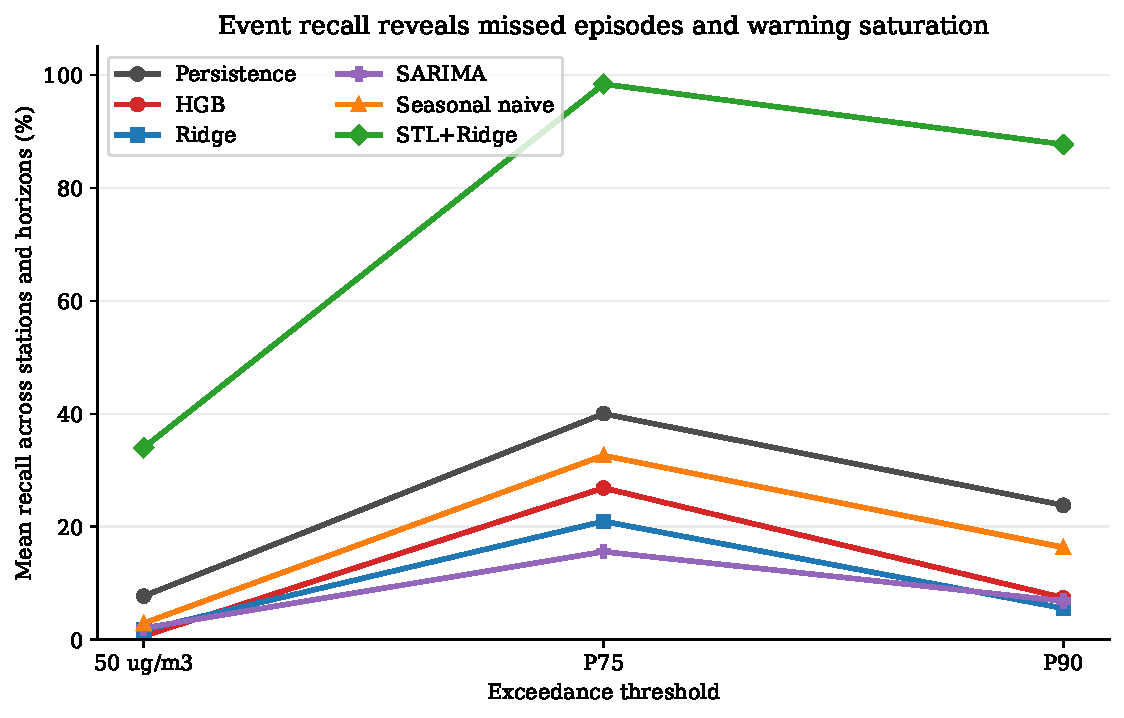
\includegraphics[width=\linewidth]{figures/figure_exceedance_recall.pdf}
  \caption{Mean exceedance recall across stations and horizons. Despite positive RMSE skill, HGB, Ridge, and SARIMA miss many P75 and P90 events. STL+Ridge attains high recall, but this must be interpreted together with its low precision and high false-alarm rate.}
  \label{fig:exceedance_recall}
\end{figure}

\subsection{Murphy decomposition}

The Murphy decomposition links the empirical findings to forecast verification theory \cite{murphy1988}. The smoothed models reduce error while compressing predictive variability, whereas STL+Ridge preserves or inflates variability but introduces large error components. This decomposition supports the interpretation that the main failure mode is not simple unconditional bias but a mismatch between forecast amplitude, phase, and conditional structure.

\begin{figure}[t]
  \centering
  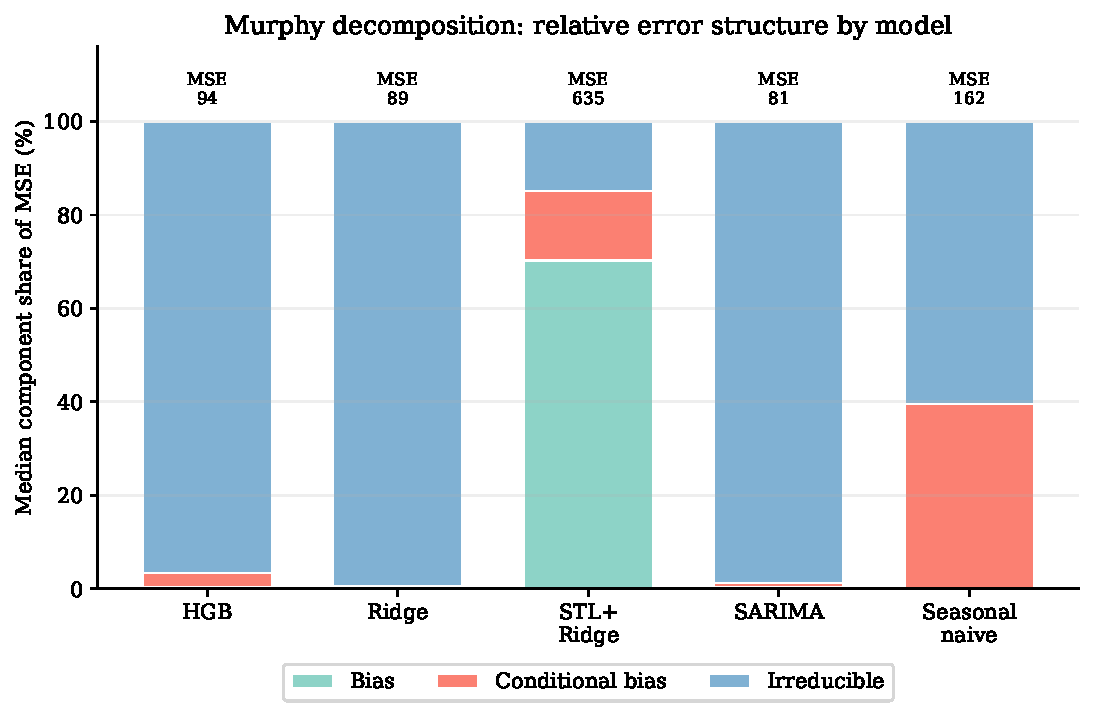
\includegraphics[width=\linewidth]{figures/figure_murphy_decomposition.pdf}
  \caption{Murphy decomposition of mean squared error by model. Bars show median percentage contribution of bias, conditional bias, and irreducible components; labels above bars report median MSE. The decomposition shows that variance preservation alone does not guarantee useful deterministic forecasts.}
  \label{fig:murphy_decomposition}
\end{figure}

\subsection{Cross-station consistency and station heterogeneity}
\label{E3}

The station set is heterogeneous, including urban traffic, urban/background, suburban industrial, rural remote/background, and EMEP sites. Figure~\ref{fig:station_map_ml_only} shows the geographic distribution and confirms that variance collapse in direct ML is nearly ubiquitous across station types.

\begin{figure}[t]
  \centering
  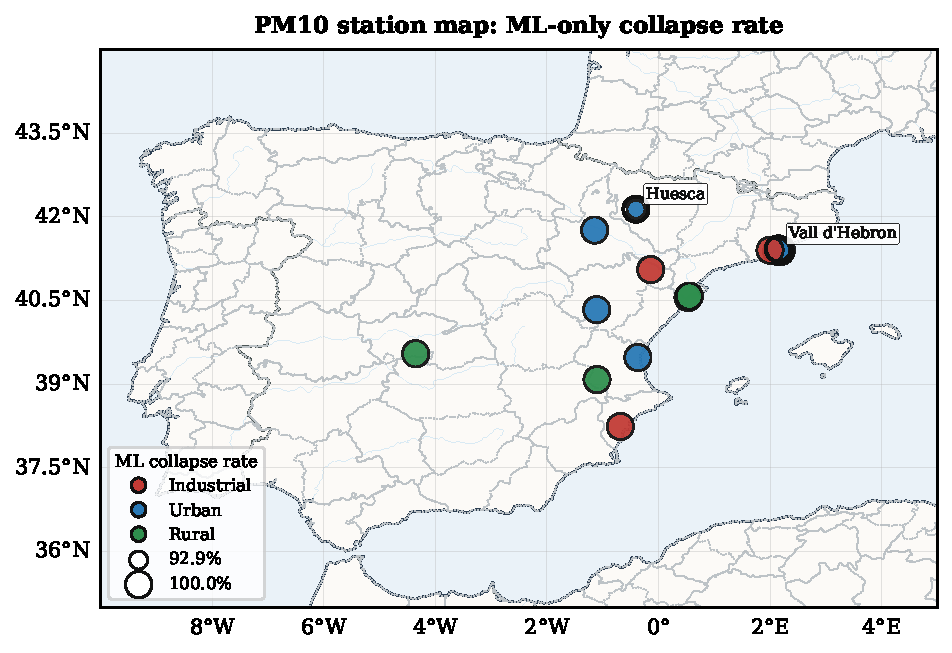
\includegraphics[width=\linewidth]{figures/station_map_ml_only_collapse_rate.pdf}
  \caption{Geographic distribution of the 17 MITECO stations. Marker colour denotes station type. Marker size denotes the ML-only collapse rate, computed over 14 model-horizon cells per station (2 direct ML models x 7 horizons). Fifteen stations show 14/14 collapsed ML cells; Huesca and Barcelona Vall d'Hebron show 13/14 due to one non-collapsed h=1 cell each.}
  \label{fig:station_map_ml_only}
\end{figure}

The results set an operational paradox: the direct ML forecasters can improve upon persistence in RMSE while producing trajectories that are substantially smoother than the observations. Interpreting performance therefore requires separating baseline-relative error reduction from the extent to which forecasts preserve day-to-day variability across horizons. The following discussion connects this decoupling to the squared-error objective and clarifies what it implies for episode-sensitive use.


\section{Discussion}
\label{sec:discussion}

The central result is a decision consequence: in this benchmark, 269 of 277 cells that pass the conventional error-based rule do not pass the added fidelity requirements. The audit therefore exposes a difference between being better than persistence under RMSE and retaining the observed variance of the forecast trajectory.

The discordant cells clarify the practical meaning of that difference. A model can pass the error and P75-recall screens while producing a forecast with $\alpha<0.50$. Conversely, seasonal naive retains variance but is rarely error-eligible, while STL+Ridge avoids collapse at the cost of poor error skill. These profiles show why error and fidelity should be reported together when model selection is intended to support dynamic episode decisions.

The Rule-B thresholds are deliberately operational. Their purpose here is sensitivity of the eligibility decision, not prescription of a universal standard. The appropriate fidelity threshold depends on the decision, pollutant, lead time, and tolerance for missed episodes or false alarms. The result supports an auditable multi-dimensional reporting practice, not a new metric or a replacement for RMSE.

\subsection{Limitations}
The evidence is bounded to daily PM$_{10}$ from 17 Spanish monitoring stations, five model families, seven horizons, and a rolling-origin benchmark. The 595 cells share stations and underlying series and are not independent replicates. Rule-B thresholds are study-specific. The aggregate evidence is recovered and frozen; the row-level manifest notes that SARIMA skill is not independently reconstructable cell-by-cell from the distributed combined row-level file alone. The analysis uses deterministic point forecasts, does not establish causal explanations for variance collapse, and does not establish generalisation to other pollutants, countries, temporal resolutions, horizons, or model families.

\section{Conclusions}
\label{sec:conclusions}

In a 595-cell, multi-station daily PM$_{10}$ benchmark, conventional error-based eligibility identified 277 cells, while adding two explicit dynamic-fidelity criteria left 8. The 269 changed statuses amount to 97.1\% of the cells eligible under Rule A, and 101 cells met the study's descriptive discordance definition.

The methodological implication is narrow but actionable: persistence-relative error skill and dynamic fidelity answer different verification questions. Model-selection reports should make that distinction visible and state any fidelity thresholds as decision-specific conventions. These conclusions apply to the evaluated stations, models, horizons, and non-independent cell structure; they are not a universal claim about forecasting systems.


\section*{CRediT author statement}
\textbf{Federico Garc\'ia Crespi:} Conceptualisation, Data curation, Formal analysis, Investigation, Methodology, Software, Validation, Visualisation, Writing -- original draft, Writing -- review \& editing. \textbf{Julio Alberto Ramos Mart\'inez:} Conceptualisation, Supervision, Writing -- review \& editing.

\section*{Declaration of competing interest}
The authors declare that they have no known competing financial interests or personal relationships that could have appeared to influence the work reported in this paper.

\section*{Data Availability Statement}
Raw daily PM$_{10}$ observations were obtained from the MITECO Spanish national air-quality network portal (\url{https://www.miteco.gob.es/}) and are publicly available. The analysis code, processed per-station series, and the 595-cell aggregate diagnostic tables (variance retention, Diebold--Mariano significance, exceedance, Murphy decomposition) underlying every multi-station figure are version-controlled at \url{https://github.com/fedeg-umh-es/varret-pm10-paper} under \texttt{evidence/paper\_a/}, with SHA-256 checksums and provenance recorded in \texttt{evidence/paper\_a/manifests/provenance\_manifest.csv}. The row-level prediction set (895{,}737 rows spanning all 17 stations, 5 model families, and 7 horizons) is available as a versioned GitHub release asset of the same repository (tag \texttt{paper-a-row-level-evidence-v1}), with its SHA-256 checksum reported in \texttt{evidence/paper\_a/row\_level/predictions\_all\_stations\_manifest.md} and in the release notes.

\section*{Acknowledgments}
The authors used a generative AI assistant for language editing and for \LaTeX\ and reference formatting. All data processing, analysis, results, and scientific conclusions are the authors' own and were verified by the authors, who take full responsibility for the content of this paper.
This research received no specific grant from funding agencies in the public, commercial, or not-for-profit sectors.

\section*{Supplementary Material}
% Supplementary material for the multi-station PM10 eligibility audit.

\subsection*{S1. Monitoring stations}
\begin{table}[ht]
\centering
\small
\setlength{\tabcolsep}{3pt}
\caption{Monitoring stations represented in the recovered station metadata. The table is descriptive and does not introduce additional empirical rows beyond the canonical 595-cell benchmark.}
\label{tab:stations-supp}
\begin{tabular}{@{}l>{\raggedright\arraybackslash}p{3.8cm}>{\raggedright\arraybackslash}p{3.3cm}rr@{}}
\hline
Station code & Name & Area type & Altitude (m a.s.l.) & Coverage (\%) \\
\hline
ES0446A & Elx-Agroalimentari & Suburban/Industrial & 44 & 80.4 \\
ES1619A & Valencia-Vivers & Urban/Residential & 11 & 91.7 \\
ES0012R & Zarra-EMEP & Rural Remote EMEP & 855 & 96.0 \\
ES1870A & Barcelona El Port Vell & Suburban/Industrial & 1 & 98.5 \\
ES1418A & Alagon & Suburban/Traffic & 235 & 97.5 \\
ES1421A & Teruel & Urban/Background & 915 & 96.7 \\
ES0001R & San Pablo de los Montes & Rural Remote/Background & 923 & 96.1 \\
ES1438A & Barcelona L'Eixample & Urban/Traffic & 26 & 95.3 \\
ES0567A & Barcelona Zona Universitaria & Urban/Background & 24 & 95.2 \\
ES1417A & Huesca & Urban/Traffic & 488 & 95.0 \\
ES0691A & Barcelona El Poblenou & Urban/Background & 3 & 94.9 \\
ES0559A & Barcelona Pl. Universitat & Urban/Traffic & 24 & 94.9 \\
ES1856A & Barcelona Vall d'Hebron & Urban/Background & 136 & 94.5 \\
ES1966A & Alcaniz Capuchinos & Urban/Industrial & 340 & 94.3 \\
ES2011A & Sant Vicenc dels Horts Alaba & Suburban/Industrial & 65 & 94.1 \\
ES2091A & Alcanar Montecarlo & Rural Remote/Industrial & 6 & 93.7 \\
ES2017A & Alcanar Llar de Jubilats & Rural Near-city/Industrial & 7 & 93.6 \\
\hline
\end{tabular}
\end{table}


\bibliographystyle{elsarticle-num-names}
\bibliography{references}

\end{document}
